\chapter{几何促进的3D分子图生成(GFMDiff)}
\label{chap:gfmdiff}

在本节中,本文将着重介绍创新3D药物分子设计的模型框架,具体包括本文提出的E(n)等变去噪内核,几何信息促进的损失函数,扩散及去噪过程和优化目标。本文提出的创新3D药物分子设计整体框架GFMDiff由图~\ref{fig:gfmdiff}~所示。

\begin{figure}[h]
    \centering
    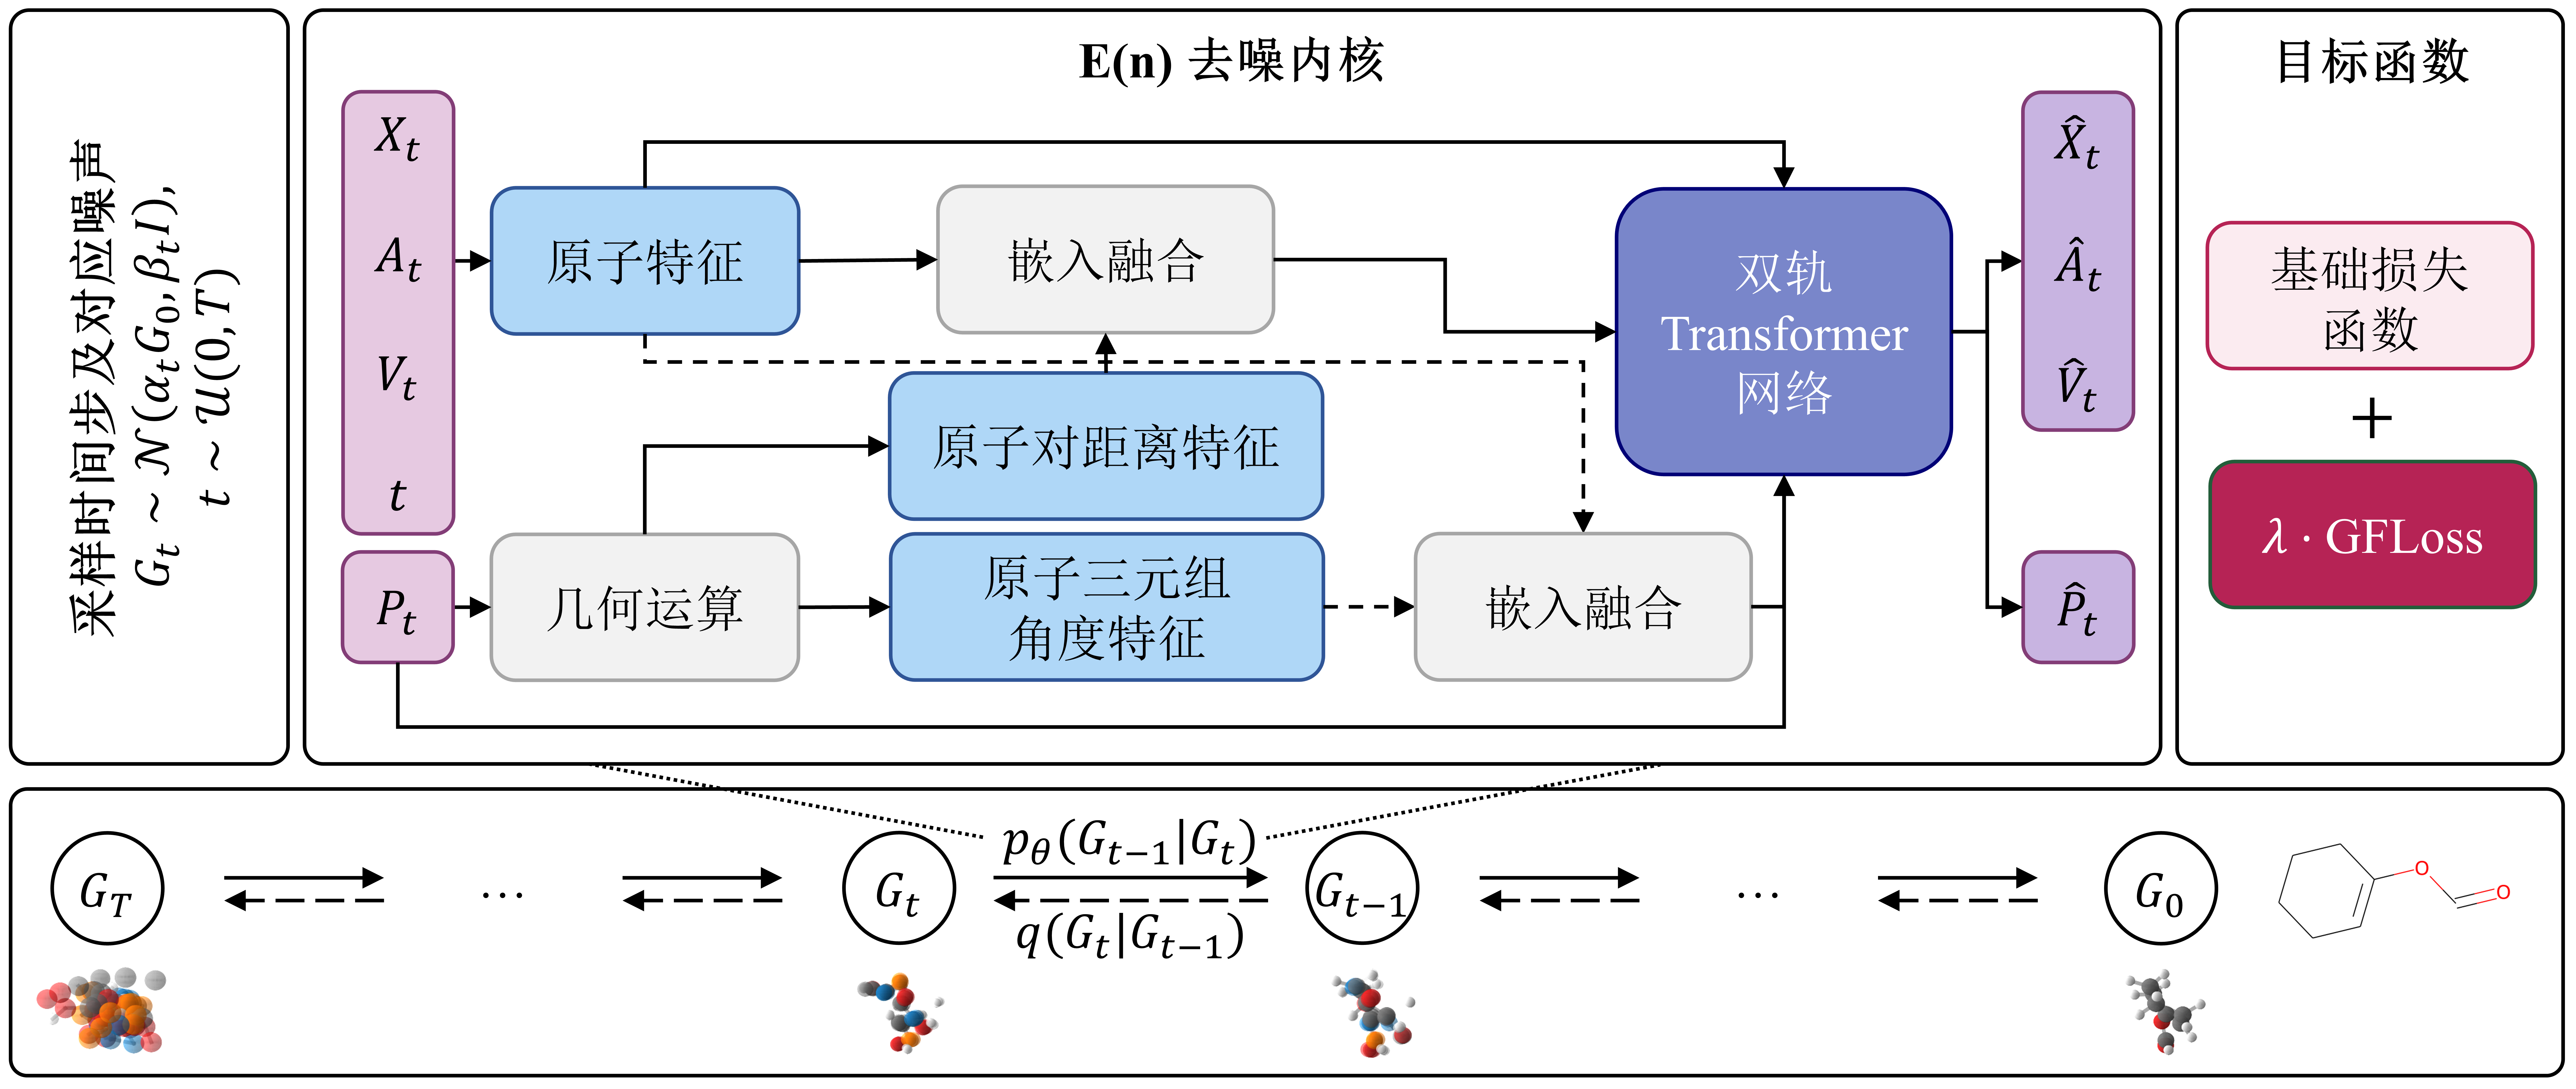
\includegraphics[width=\linewidth]{figures/overview_gfmdiff.png}
    \caption{GFMDiff模型框架示意图}
    \label{fig:gfmdiff}
\end{figure} 

对于每个训练样本,模型的输入为随机选取的时间步$t$和采样自对应时刻噪声分布的样本。通过几何计算及编码,得到的原子特征,原子对距离特征,三元组角度特征将被用于E(n)等变的去噪内核DTN中的分子学习,并得到更新后的样本在$t-1$时刻的分布,即对应的原子特征和位置信息。

\section{双轨Transformer网络(DTN)}
在这个小节中,我们将详细介绍作为GFMDiff的E(n)等变去噪内核的双轨Transformer网络(Dual-track Transformer Network / DTN)。DTN被设计用于有效捕捉原子之间的关系和原子特征。由于三维分子几何具有旋转、平移、反射和排列等不变性质,使得去噪核满足这些性质是很重要的。本文所提出的DTN不仅是E(n)等变的,还能充分利用空间信息,进而预测高质量的原子及分子特征。图~\ref{fig:dtn}~为DTN的模型结构。

\begin{figure}[h]
  \centering
  
\includegraphics[width=\linewidth]{figures/structure_dtn.png}
  \caption{DTN去噪内核结构示意图}
  \label{fig:dtn}
\end{figure}

% 传统的图神经网络用于学习图结构数据的拓扑信息,仅仅是置换等变的。尽管已经有许多努力致力于赋予GNN上述性质,我们提供了另一种解决这个问题的视角。

在我们提出的方法中,我们将具有总原子数$N$的输入分子视为$G = (P, X, A, V)$,其中$P = (p_1, p_2, ..., p_N) \in \mathbb{R}^{N \times 3}$表示原子坐标,$X = (x_1, x_2, ..., x_N) \in \mathbb{R}^{N \times nf}$表示原子编号的独热编码,$A = (a_1, a_2, ..., a_N) \in \mathbb{R}^{N}$表示原子编号,$V = (v_1, v_2, ..., v_N) \in \mathbb{R}^{N}$表示原子化合价数。为了确保等变性,DTN利用原子对距离信息和三元组角度信息捕捉几何信息。原子$i$和$j$之间的欧几里得距离反映了原子间相互作用的强度,可以通过以下公式获得:
\begin{equation}
    d_{ij} = ||p_i - p_j||_2.
\end{equation}
在分子中,除了氢原子,其他多数原子能够形成超过一个单键,故存在大量原子间的多体复杂关系。因此仅使用原子对距离是不足以充分提取空间几何信息。本文提出进一步使用以下公式计算原子三元组间的夹角:
\begin{equation}
    \varphi_{ijk} = \arccos \left(\frac{(p_i - p_j) \times (p_i - p_k)}{||p_i - p_j||_2 \times ||p_i - p_k||_2} \right). 
\end{equation}
经过上述几何计算,本文通过径向基神经网络(Radial Basis Function / RBF)编码得到可以被用作神经网络学习的原子对距离特征和三元组角度特征:
\begin{eqnarray}
    &e_{ij} = {\rm Linear}({\rm RBF}(d_{ij}), e_i, e_j),& \\
    &e_{ijk} = {\rm Linear}({\rm RBF}(\varphi_{ijk}), e_i, e_j, e_k),&
\end{eqnarray}
其中$e_i = {\rm Embedding}(x_i, a_i, v_i)$是原子$i$的节点嵌入,由原子序数和化合价决定。这些特征随后被输入到$L$层的DTN中。RBF函数是一种常用的径向基函数。在机器学习和模式识别领域中,RBF函数常用于对数据进行特征编码和表征,以距离特征计算为例:
\begin{eqnarray}
    &K(d_{ij}, \mu_k) = {\rm exp} \left(- \frac{||d_{ij} - \mu_k||^2}{2\sigma^2}\right), & \\
    &{\rm RBF}(d_ij) = {\rm Linear}(K(d_{ij}, \mu_k)), &
\end{eqnarray}
其中中心$\mu_k$和自由参数$\sigma$为RBF函数参数。在距离特征计算时,$\mu$满足$0 \text{\AA} \leq \mu_k \leq 10 \text{\AA}$并以$0.2\text{\AA}$的间隔切片,$\sigma$满足$\frac{1}{2\sigma^2} = 10 \text{\AA}$。经过切片操作后,$K(d_{ij}, \mu_k)$的维度为50,故需要通过线性层将RBF特征映射到与原子对特征维度一致的高位特征空间内。在角度计算时,$\mu$满足$0 \text{\AA} \leq \mu_k \leq \pi \text{\AA}$并以$0.1\text{\AA}$的间隔切片,$\sigma$满足$\frac{1}{2\sigma^2} = 10 \text{\AA}$。

DTN的每一层由以下组件组成:原子-原子对轨道、原子对-三元组轨道和连接模块。原子-原子对轨道模拟了原子之间的相互作用力对目标原子的影响,而原子对-三元组轨道则模拟了键角对边潜在的影响。连接模块作为两个轨道之间的桥梁,将原子特征注入到原子对特征中,以促进更好的表示学习。

原子-原子对轨道预测其他原子和原子之间相互作用力对目标原子的影响。该轨道将原子嵌入$e_i$和原子对嵌入$e_{ij}$作为输入,其中用于更新原子特征的多头注意力机制模块为:
\begin{eqnarray}
    &e_i = {\rm LayerNorm}(e_i),& \\
    &e_{ij} = {\rm LayerNorm}(e_{ij}),& \\
    &\mathbf{Q}_i = {\rm Linear}(e_i),& \\ 
    &\mathbf{K}_i = {\rm Linear}(e_i) + {\rm Linear}(e_{ij}),& \\
    &a_i = {\rm Dropout} \left({\rm softmax} \frac{\mathbf{Q}_i \mathbf{K}_i^T}{\sqrt{d_h}} \right), & \\
    &\mathbf{V}_i = {\rm Linear}(e_{ij}) + {\rm Linear}(e_{i}) + {\rm Linear}(e_{j}),& \\
    &\hat{e}_i = {\rm Linear}(a_i \mathbf{V}_i^T),&
\end{eqnarray}
其中$d_h$是多头注意力机制的头的数量。原子嵌入首先通过原子-原子对轨道输出的原子嵌入相加的方式更新,然后通过给前馈网络。在每一层DTN中,原子会接收来自于其他原子和相应的原子对的信息。

类似地,原子对-三元组轨道预测了复杂几何亚结构对原子间相互作用力的影响。其中的多头注意力机制模块可以表示为:
\begin{eqnarray}
    &e_{ij} = {\rm LayerNorm}(e_{ij}),&\\
    &e_{ijk} = {\rm LayerNorm}(e_{ijk}),&\\
    &\mathbf{Q}_{ij} = {\rm Linear}(e_{ij}),& \\ 
    &\mathbf{K}_{ij} = {\rm Linear}(e_{ij}) + {\rm Linear}(e_{ijk}),& \\
    &a_{ij}= {\rm Dropout} \left({\rm softmax} \frac{\mathbf{Q}_{ij} \mathbf{K}_{ij}^T}{\sqrt{d_h}} \right), & \\
    &\mathbf{V}_{ij} = {\rm Linear}(e_{ij}) + {\rm Linear}(e_{ijk}),& \\
    &\hat{e}_{ij} = {\rm Linear}(a_{ij} \mathbf{V}_{ij}^T).&
\end{eqnarray}
值得注意的是,三元组嵌入$e_{ijk}$在Transformer结构中不会得到更新,因为这会显著增加计算资源的需求。它们只会在原子坐标更新时利用特征编码得到更新。

连接模块的作用是将原子嵌入融合到原子对嵌入中。对于原子对嵌入$e_{ij}$,它同时接收来自连接模块的原子特征信息和来自原子对-三元组轨道的局部空间信息。
\begin{equation}
    e_{ij} = {\rm LayerNorm}(e_{ij} + {\rm Linear}({\rm Linear}(e_i) \otimes {\rm Linear}(e_j)))
\end{equation}

在更新坐标的方法上,我们遵循EDM \cite{edm_hoogeboom_22}和MDM \cite{mdm_huang_23}中的相关设计。
\begin{equation}
    \hat{p}_i = p_i + \sum_{j \neq i} \frac{p_i - p_j}{d_{ij} + 1} {\rm Linear}(\hat{e}_i, \hat{e}_j, d_{ij}^2, \hat{e}_{ij})
\end{equation}

由于在该坐标更新模块中,仅依赖于原子间相对距离更新原子坐标,故其严格遵循E(n)等变性要求。在原子坐标得到更新后,原子对和原子三元组的嵌入也将得到更新:
\begin{eqnarray}
  &e_{ij} = {\rm Linear}[{\rm Linear}({\rm RBF}(\hat{d}_{ij}), \hat{e}_{ij}), \hat{e}_i, \hat{e_j}],& \\
  &e_{ijk} = {\rm Linear}({\rm RBF}(\hat{\varphi}_{ijk}), e_{ijk}). &
\end{eqnarray}

更新后的原子对距离特征和三元组角度特征可以被用作下一层DTN网络的输入,或是直接作为去噪内核的输出。运用该种方法能够避免通过神经网络直接更新三元组嵌入,故而在极大减小计算需求的同时,又能通过简单的线性层更新能够反映几何特征的三元组特征。在算法~\ref{alg:dtn}~中详细的介绍了每一层的DTN的计算流程。

\begin{algorithm}[t]
    \caption{DTN去噪内核伪代码}
    \label{alg:dtn}
    \begin{algorithmic}
    \STATE {\bfseries Input} 原子特征$e_i$,原子对特征$e_{ij}$,三元组特征分子$e_{ijk}$和几何坐标$p_t$;
    \STATE 层归一化$e_i$和$e_{ij}$;
    \STATE 计算多头注意力概率$a_i$和值$\mathbf{V}_i$;
    \STATE 得到更新的原子特征残差$\hat{e}_i$并更新原子特征$e_i$;
    \STATE 通过连接模块将原子特征计$e_i$融入原子对特征$e_{ij}$;
    \STATE 层归一化$e_{ij}$和$e_{ijk}$;
    \STATE 计算多头注意力概率$a_{ij}$和值$\mathbf{V}_{ij}$;
    \STATE 得到更新的原子特征残差$\hat{e}_{ij}$并更新原子特征$e_{ij}$;
    \STATE 通过坐标更新模块更新坐标$\hat{p}_t$;
    \STATE 进行几何计算,并对新的原子对特征$e_{ij}$和三元组特征$e_{ijk}$进行编码;
    \STATE {\bfseries Return} 新的原子特征$e_i$,原子对特征$e_{ij}$,三元组特征分子$e_{ijk}$和几何坐标$p_t$.
    \end{algorithmic}
\end{algorithm}

\section{几何信息促进的损失函数(GFLoss)}
预测化学键的存在是分子图生成中的基本且不可或缺的任务。与以往的研究完全依赖于预设规则生成边的范式不同,我们提出在训练过程中积极干预化学键的形成,通过设计一种精细的训练目标函数,命名为几何促进损失(Geometric-facilitated Loss / GFLoss),以高效的方式干预边的形成。这个损失函数的目的是引导模型生成既具有有效的拓扑结构,又具有稳定构象的分子。在药物分子设计中,我们认为原子的价是一种非常重要的辅助特征类型。因此,在上述提到的分子学习网络DTN中,原子的价被作为原子特征的一部分进行了整合。这使得模型能够学习和利用原子的价信息,具体计算流程和伪代码如图~\ref{fig:gfloss}~和算法~\ref{alg:gfloss}~所示。

\begin{figure}[h]
    \centering
    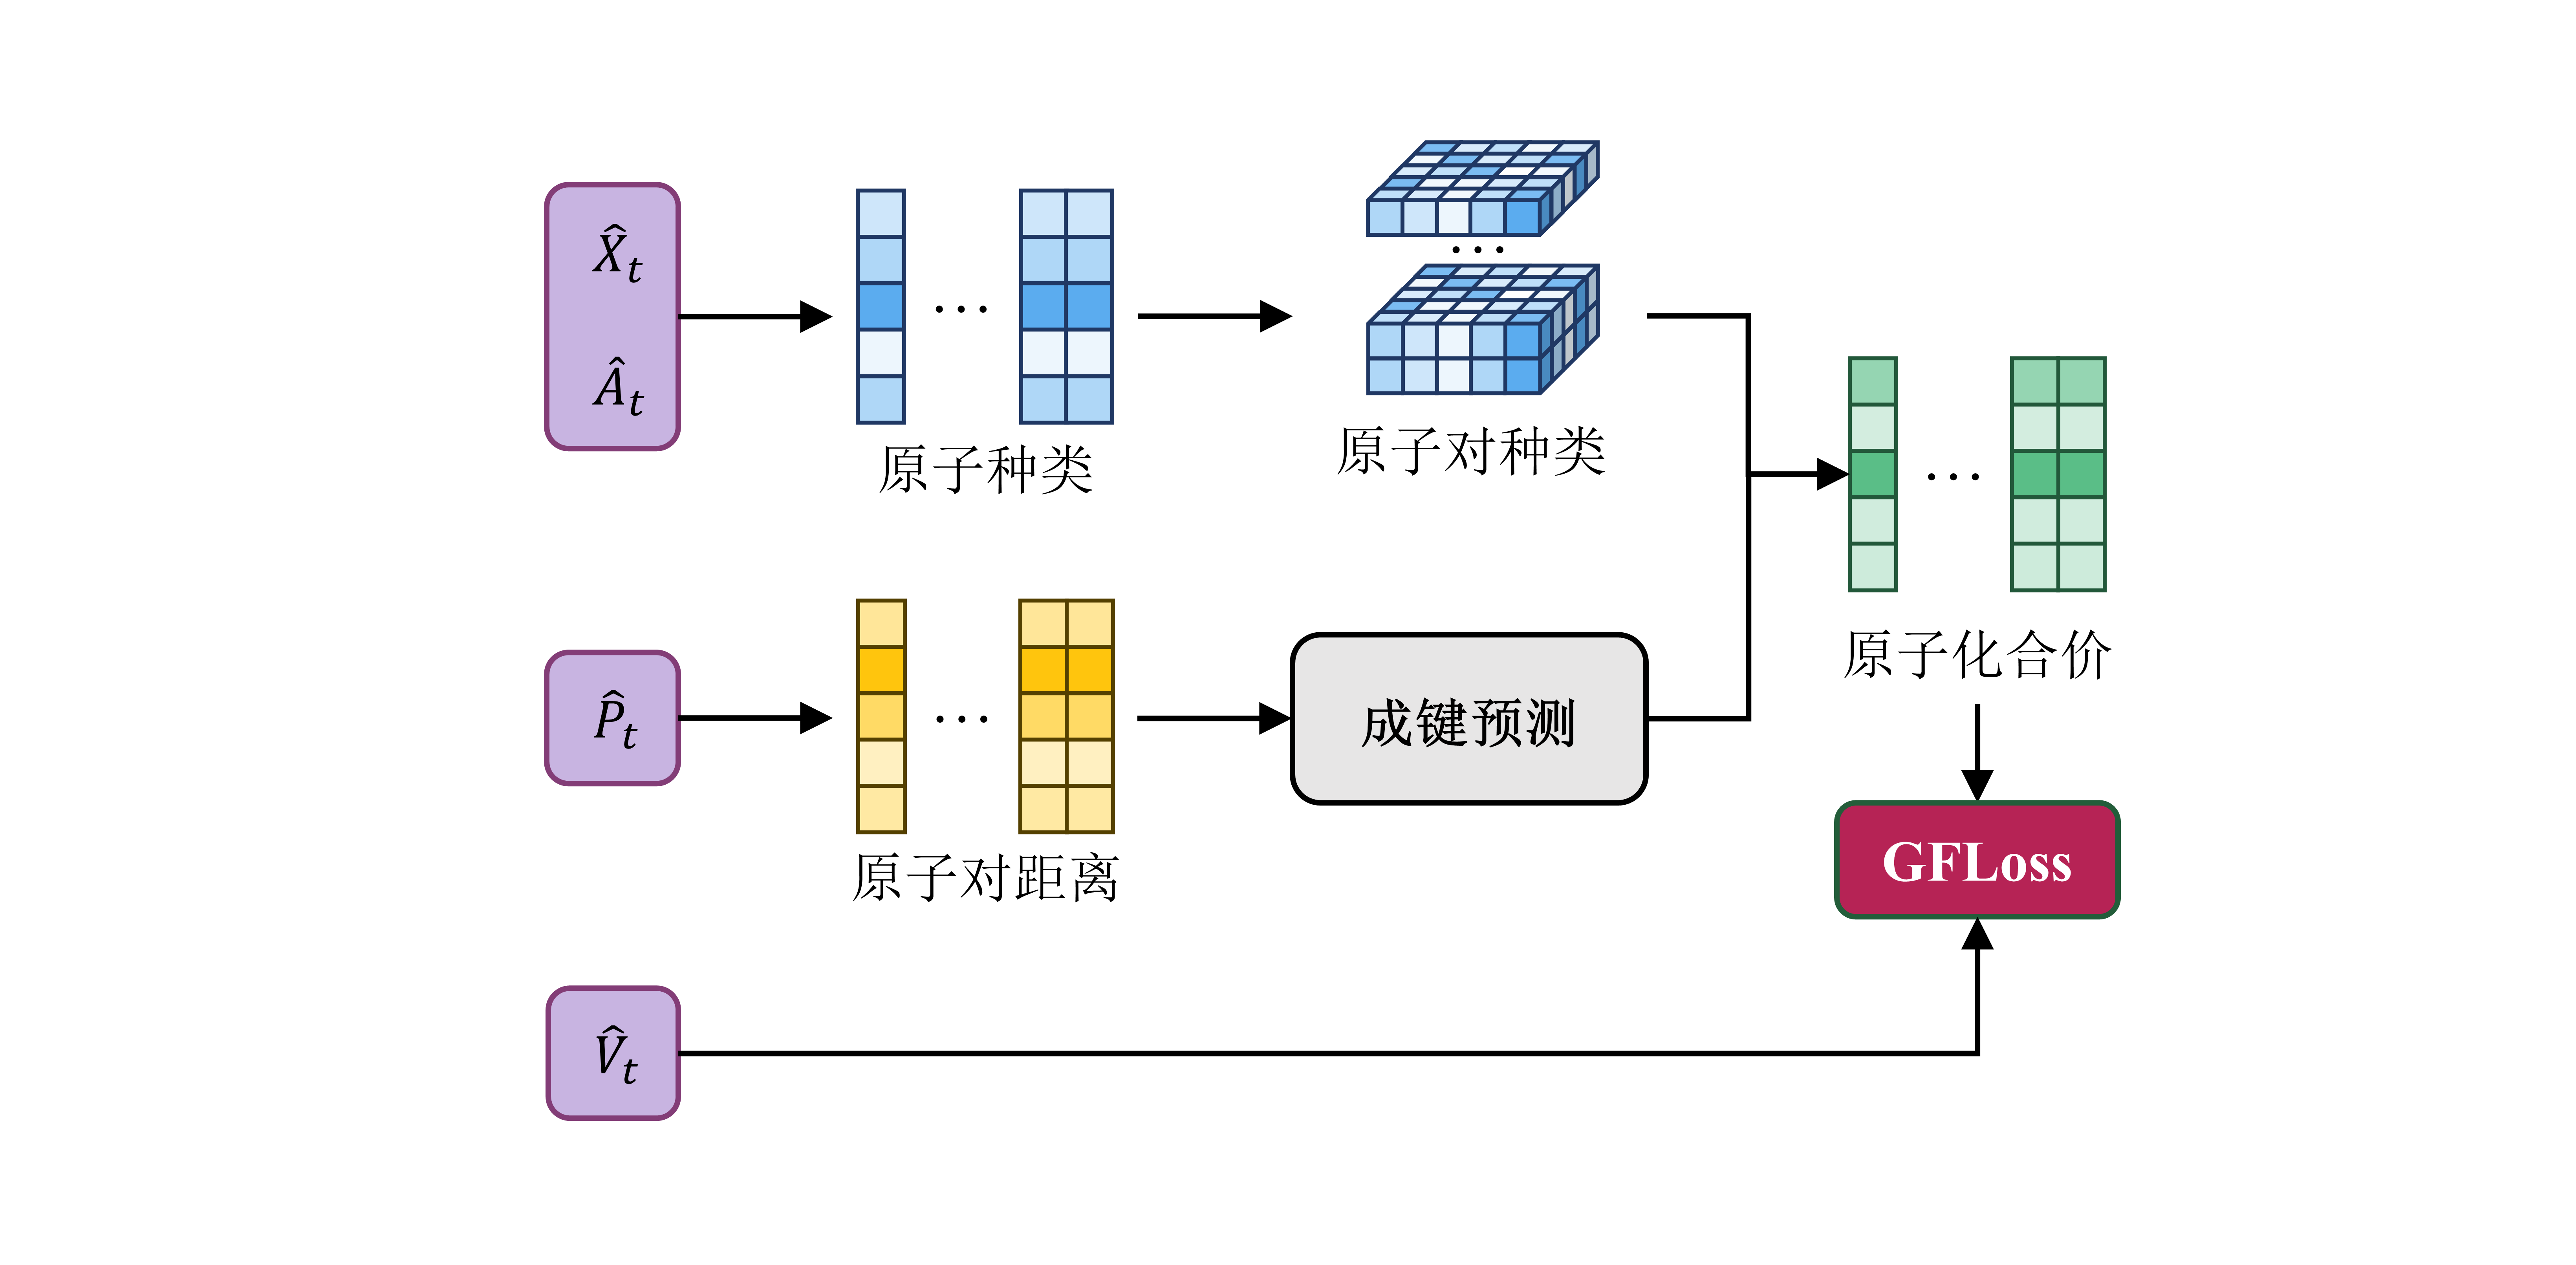
\includegraphics[width=\linewidth]{figures/gfloss.png}
    \caption{GFLoss损失函数}
    \label{fig:gfloss}
\end{figure} 

根据预定义的规则,具有适当距离的原子对间被认为有化学键的存在。对于单键、双键或三键,特定种类的原子之间存在典型距离。如果一对原子之间的距离在某个范围内,这两个原子被认为是由对应类型的键连接的。假设预定义的距离和边界为 $\mathbf{D} \in \mathbb{R}^{nf \times nf \times 3}$ 和 $\mathbf{M} \in \mathbb{R}^{3}$,其中3表示键的类型数量。基于 DTN 的输出 $\hat{G}_t = (\hat{P}_t, \hat{X}_t, \hat{A}_t, \hat{V}_t)$,我们首先使用softmax函数预测原子类型的概率:
\begin{equation}
    {\mathbf{p}}_t(\hat{X}_{{\rm atom}}) = {\rm softmax}(\hat{X}_t) \in \mathbb{R}^{N \times nf},
\end{equation}
其中 $\hat{X}_t$ 在此处表示维度为 $nf$ 的独热编码格式的预测原子类型。原子对的原子类型概率为:
\begin{equation}
    {\mathbf{p}}_t(\hat{X}_{{\rm pair}}) = {\mathbf{p}}_t(\hat{X}_{{\rm atom}}) \cdot {\mathbf{p}}_t(\hat{X}_{{\rm atom}}) \in \mathbb{R}^{N \times N \times nf \times nf}.
\end{equation}

利用DTN预测的原子坐标 $\hat{P}_t$,可以得到原子对距离矩阵 $\mathbf{d}_t \in \mathbb{R}^{N \times N}$,为了方便后续计算,在此需要将其扩展到 $\mathbb{R}^{N \times N \times nf \times nf \times 3}$。为了判断键的存在性,原子对间距与典型的键距离之间的差距 $\mathbf{m}_t$ 计算如下:
\begin{equation}
    \mathbf{m}_t = \mathbf{d}_t - (\mathbf{D} + \mathbf{M}) \in \mathbb{R}^{N \times N \times nf \times nf \times 3}.
\end{equation}
以原子 $i$ 和 $j$ 为例,假设它们被认为是碳原子的概率大于零,如果差距$\mathbf{m}_t(i,j,{\rm C},{\rm C},:)$ 中的任一元素小于零,则表示原子 $i$ 和 $j$ 之间存在一条化学键。化学键的具体类型由差距 $\mathbf{m}_t(i,j,{\rm C},{\rm C},:)$ 中最小值的索引确定。如果 $\arg\min (\mathbf{m}_t(i,j,{\rm C},{\rm C},:))$ 为 1,则化学键判定为单键。如果 $\arg\min (\mathbf{m}_t(i,j,{\rm C},{\rm C},:))$ 为 3,则化学键判定为三键。表示键存在性的布尔矩阵记为 ${\rm ISBOND}_t \in \mathbb{R}^{N \times N \times nf \times nf}$。

一旦我们获得了原子对的原子类型概率和键的存在性预测,就可以估计几何构象决定的原子可能化合价:
\begin{equation}
     \hat{V}_{{\rm pred}}(t) = {\rm sum}({\mathbf{p}}_t(\hat{X}_{{\rm pair}}) \odot {\rm ISBOND}_t) \in \mathbb{R}^{N}.
\end{equation}
由于输入数据受到不同水平噪声的影响,GFLoss被定义为$t$时刻几何构象决定的化合价 $V_{{\rm pred}}(t)$ 与输入样本的真实化合价 $V_t$ 之间的均方误差:
\begin{equation}
    \mathcal{L}_{GF}(t) = ||\alpha_t(\hat{V}_{{\rm pred}}(t) - V_t)||^2,
\end{equation}
其中 $\alpha_t$ 是扩散过程中噪声数据中真实数据的水平。

\begin{algorithm}[H]
    \caption{GFLoss损失函数项伪代码}
    \label{alg:gfloss}
    \begin{algorithmic}
    \STATE {\bfseries Input} 预测的原子序数$\hat{X}_t$,化合价$\hat{V}_t$和几何坐标$\hat{P}_t$;
    \STATE 根据预测的原子序数$\hat{X}_t$计算任一原子类型${\mathbf{p}}_t(\hat{X}_{{\rm atom}})$;
    \STATE 根据任一原子类型计算任一原子对的原子类型${\mathbf{p}}_t(\hat{X}_{{\rm pair}})$;
    \STATE 计算任一原子对距离$\mathbf{d}_t$;
    \STATE 计算原子对距离与3种化学键的典型键长之间的差距$\mathbf{m}_t$;
    \STATE 根据差距$\mathbf{m}_t$判断原子对是否形成某种化学键,并记为布偶型矩阵${\rm ISBOND}_t$;
    \STATE 根据矩阵${\rm ISBOND}_t$和原子对的原子类型${\mathbf{p}}_t(\hat{X}_{{\rm pair}})$计算由几何构象和化学规则
    
    预测的原子化合价$\hat{V}_{{\rm pred}}(t)$;
    \STATE {\bfseries Return} $\mathcal{L}_{GF}(t) = ||\alpha_t(\hat{V}_{{\rm pred}}(t) - V_t)||^2$.
    \end{algorithmic}
\end{algorithm}

\section{扩散及去噪过程}
在提出的GFMDiff的前向过程中,位置、原子序数和原子价逐渐被预设定的噪声先验分布所扰动。对于任一时间步$t = 0, \ldots, T$,需要定义均值$\alpha_t$及方差序列$\sigma_t$。由于 $\alpha_t = \sqrt{1 - \sigma_t^2}$,故实际工程实践中只需定义 $\alpha_t$ 即可。伴随噪声的逐步加入,样本原有的真实信息占比也逐渐减少,故均值序列的值应该单调递减,从 $\alpha_0 \approx 1$ 开始递减,最终到达 $\alpha_T \approx 0$。在本文中,我们设定
\begin{eqnarray}
    &\alpha_t = (1 - 2s) \cdot f(t) + s, & \\
    &f(t) = (1 - (t/T)^2)& 
\end{eqnarray}

为避免数值不稳定情况,序列的数值精度$s$取 $10^{-5}$。该序列设定与\cite{impddpm_nichol_21}中引入的余弦噪声序列较为相似,但本文使用的序列在形式上更为简洁。为了避免采样过程中的数值不稳定性,我们遵循先前研究的\cite{impddpm_nichol_21}的剪切过程,并得到$\alpha_{t|t-1} = \alpha_t / \alpha_{t-1}$,其中$\alpha_{-1} = 1$。在剪切过程中,$\alpha_{t|t-1}^2$的值被剪切到下限$0.001$。这样做确保了$1 / \alpha_{t|t-1}$现在在采样过程中有界,避免采样过程中数值不稳定性。而后,$\alpha_t$ 的值可以使用累积乘积 $\alpha_t = \prod_{\tau=0}^t \alpha_{\tau|\tau-1}$来重新计算。

在方差序列中,$\mathrm{SNR}(t) = \alpha_t^2 / \sigma_t^2$。参照相关研究\cite{vaediff_kingma_21},本文计算负对数$\mathrm{SNR}$曲线为$\gamma(t) = -(\log \alpha_t^2 - \log \sigma_t^2)$,其作为一个单调递增的函数,对高精度数值计算由重要作用。例如,$\alpha_t^2 = \mathrm{sigmoid}(-\gamma(t))$,$\sigma_t^2 = \mathrm{sigmoid}(\gamma(t))$,以及 $\mathrm{SNR}(t) = \exp(-\gamma(t))$,都可以通过对$\gamma(t)$变形得到。

通过具有预定义方差序列$\beta_t \in (0, 1), t=0, 1, ..., T$的马尔可夫链将真实构象$G_0 = (P_0, X_0, A_0, V_0)$进行转换。后验分布定义为:
\begin{eqnarray}
    &q(G_{1:T}|G_0) = \prod^T_{t=1} q(G_t|G_{t-1}),& \\
    &q(G_t|G_{t-1}) = \mathcal{N}_p(p_t;\sqrt{\alpha_t} p_{t-1}, \beta_t I) \cdot \mathcal{N}_h(h_t;\sqrt{\alpha_t} h_{t-1}, \beta_t I),&
\end{eqnarray}
为方便起见,其中$h_t = {\rm concat}(x_t, a_t, v_t)$表示原子特征。

为了在去噪过程中的满足几何坐标的等变性要求,在将原子坐标引入扩散之前,它们必须先转换到质心为零的线性子空间内\cite{enf_satorras_21,edm_hoogeboom_22,geodiff_xu_22}。因此,噪声分布和上述后验分布都受限于相同的线性子空间。此外,原子特征对于对神经网络是等变的,故它们不需要进一步处理即可在整个前向和后向过程中与几何坐标一起进行运算。

考虑欧几里得变量$\mathbf{p} \in \mathbb{R}^{M \times n}$在线性子空间上满足$\sum_i \mathbf{x}_i = \mathbf{0}$。故可以认为$\mathbf{p}$是$n$维空间内的一个质心为零的点云。对于在此子空间上的一个正态分布$\mathcal{N}_x$,欧式变量服从的分布可以表示为:
\begin{equation}
    \mathcal{N}_x(\mathbf{x} | \mathbf{\mu}, \sigma^2 I) = (\sqrt{2 \pi} \sigma)^{-(M-1)\cdot n} \exp \left( -\frac{1}{2\sigma^2} || \mathbf{x} - \mathbf{\mu}||^2 \right),
\end{equation}
其中$\mathbf{\mu}$位于与$\mathbf{x}$相同的子空间中。从这个正态分布中采样有多种方法,例如可以从维度为$(M-1)\cdot n$的正态分布中采样,然后将采样映射到$M\cdot n$维的环境空间中,使得它的重心为零。但是还有一种更简单的方法:可以直接在$M\cdot n$维的环境空间中进行采样,并减去$\sum_i \mathbf{x}_i$。由于正态分布是各向同性的(即无论选择哪个方向,其方差都是 $\sigma^2$),故本文采用这样的方法对原子几何坐标进行采样。

在去噪过程中,我们使用上述的去噪核函数来逼近每个时间步的分子构象,
\begin{eqnarray}
    &p_\theta(G_{t-1}|G_t) = \mathcal{N}(G_{t-1}; \mu_\theta(G_t,t),\sigma_t^2 I),& \\
    &\hat{G}_t = G_t / \alpha_t - \hat{\epsilon}_t \times \sigma_t / \alpha_t ,&
\end{eqnarray}
其中$\hat{\epsilon}_t$是参数化神经网络的输出。

\section{目标函数与评价指标}

对于DDPMs,典型的目标函数是数据对数似然的变分下界。在先前相关研究方法的基础上,我们将目标函数与GFLoss相结合:
\begin{equation}
    \mathcal{L}_t = E_{\epsilon_t \sim \mathcal{N}(0, I)} \left[ \frac{1}{2} \omega(t) \left( ||\epsilon_t - \hat{\epsilon}_t||^2 + \lambda || \alpha_t(\hat{V}_{pred}(t) - V_t)||^2 \right) \right],
\end{equation}
其中$\omega(t) = (1-{\rm SNR}(t)/{\rm SNR}(t-1))$。

此外,在评价模型参数的好坏时,需要比较模型学习的去噪分布于前向噪声分布的差异。该指标具体表现为参数的负对数似然函数,由于负对数似然函数无法直接计算得到,本文通过算法~\ref{alg:nll_gfmdiff}~估计该负对数似然函数的取值。

\begin{algorithm}[H]
    \caption{GFMDiff参数的负对数似然函数估计}
    \label{alg:nll_gfmdiff}
    \begin{algorithmic}
    \STATE {\bfseries Input} 原子坐标$p$,原子特征$h = [x, a, v]$,去噪神经网络$\phi$;
    \STATE 采样时间步 $t \sim \mathcal{U}(1, T)$和噪声 $\varepsilon_t = [\varepsilon^{(p)}_t, ~\varepsilon^{(h)}_t] \sim \mathcal{N}(\mathbf{0}, I)$;
    \STATE 混合输入样本与噪声 $z_t = \alpha_t [p, h] + \sigma_t \varepsilon_t$;
    \STATE 计算神经网络损失函数 $\mathcal{L}_t = \frac{1}{2}(1 - \mathrm{SNR}(t-1) / \mathrm{SNR}(t)) ||\varepsilon_t - \phi(z_t, t)||^2$;
    \STATE 采样0时刻样本噪声 $\varepsilon_0 = [\varepsilon^{(p)}_0, ~\varepsilon^{(h)}_0] \sim \mathcal{N}(\mathbf{0}, I)$;
    \STATE 混合0时刻输入样本与噪声 $z_0 = \alpha_0 [p, h] + \sigma_0 \varepsilon_0$;
    \STATE 计算0时刻损失函数 $\mathcal{L}_0 = \mathcal{L}_0^{(x)} + \mathcal{L}_0^{(h)} = -\frac{1}{2} ||\varepsilon_0 - \phi(z_0, 0)||^2 - \log Z + \log p(h | z_0^{(h)})$;
    \STATE $\mathcal{L}_{\text{base}} = -\mathrm{KL}(q(z_T | x, h) | p(z_T)) = -\mathrm{KL}(\mathcal{N}_{xh}(\alpha_T [x, h], \sigma_T^2 I) | \mathcal{N}_{xh}(\mathbf{0}, I))$;
    \STATE {\bfseries Return} $\hat{\mathcal{L}} = T \cdot \mathcal{L}_t + \mathcal{L}_0 + \mathcal{L}_{\text{base}}$.
    \end{algorithmic}
\end{algorithm}

其中对于前向和反向过程的样本KL散度的计算,无法直接得到。对于两个各向同性正态分布$q = \mathcal{N}(\mathbf{\mu}_1, \sigma_1^2 I)$和$p = \mathcal{N}(\mathbf{\mu}_2, \sigma_2^2 I)$,标准的KL散度可表示为:
\begin{equation}
    \mathrm{KL}(q || p) = d \cdot \log \frac{\sigma_2}{\sigma_1} + \frac{1}{2} \left[ \frac{d \cdot \sigma_1^2 + ||\mathbf{\mu}_1 - \mathbf{\mu}_2||^2}{\sigma_2^2} - d  \right],
\end{equation}
其中$d$是分布的维度。在扩散模型中,扩散过程和去噪过程具有相同的方差$\sigma^2$。如果$\sigma_1 = \sigma_2 = \sigma$,则这两个分布的KL散度可简化为:
\begin{equation}
    \mathrm{KL}(q || p) = \frac{1}{2} \left[ \frac{||\mathbf{\mu}_1 - \mathbf{\mu}_2||^2}{\sigma^2} \right].
    \label{eqn:kl1}
\end{equation}

现假设$\mathcal{N}_1(\tilde{\mathbf{\mu}}_1, \sigma^2 I)$和$\mathcal{N}_2(\tilde{\mathbf{\mu}}_2, \sigma^2 I)$在一个线性子空间上,其中均值 $\tilde{\mathbf{\mu}}$ 是相对于子空间中的任意坐标系定义的,则这两个分布之间的KL散度包含一个包含欧几里得距离项$||\tilde{\mathbf{\mu}}_1 - \tilde{\mathbf{\mu}}_2||^2$。

类似于E-NF\cite{enf_satorras_21}和GeoDiff\cite{geodiff_xu_22}中的论证,可以构造一个正交变换$Q$,将满足$\sum_i \mathbf{\mu}_i = \mathbf{0}$条件的环境空间映射到子空间上,以满足$\begin{bmatrix} \tilde{\mathbf{\mu}} \\ \mathbf{0} \end{bmatrix} = Q \mathbf{\mu}$。由于$||\tilde{\mathbf{\mu}}|| = ||\begin{bmatrix} \tilde{\mathbf{\mu}} \\ \mathbf{0} \end{bmatrix}|| = ||\mathbf{\mu}||$,故$||\tilde{\mathbf{\mu}}_1 - \tilde{\mathbf{\mu}}_2||^2 = ||\mathbf{\mu}_1 - \mathbf{\mu}_2||^2$。这表明式~\ref{eqn:kl1}~在环境空间内可以通过计算得到。
% 这同样表明在某些扩散模型中,后验扩散过程和去噪过程使用的方差不同。从方程可以看出,KL散度取决于子空间的维度,而不是环境空间的维度。

对于诸如$\mathcal{N}$这样的分布,只要两个分布之间的方差相同,KL散度仍然可以在环境空间中计算。现在考虑分布$q = \mathcal{N}_{ph}(\mathbf{\mu}_1, \sigma^2 I)$和$p = \mathcal{N}_{ph}(\mathbf{\mu}_2, \sigma^2 I)$ 的组合KL散度。注意到这里的均值由两部分组成 $\mathbf{\mu} = [\mathbf{\mu}^{(p)}, \mathbf{\mu}^{(h)}]$,其中$p$部分位于一个子空间中,而$h$作为原子特征分布没有特定要求。因此该分布可以分解为$\mathcal{N}_{ph}(\mathbf{\mu}, \sigma^2 I) = \mathcal{N}_{p}(\mathbf{\mu}^{(p)}, \sigma^2 I) \cdot \mathcal{N}(\mathbf{\mu}^{(h)}, \sigma^2 I)$。因此扩散和去噪过程样本分布的KL散度可以被简化为:
\begin{align}
    \begin{split}
        \mathrm{KL}(q||p) &= \mathrm{KL}\left(\mathcal{N}_{p}(\mathbf{\mu}_1^{(p)}, \sigma^2 I) || \mathcal{N}_{p}(\mathbf{\mu}_2^{(p)}, \sigma^2 I)\right) + \mathrm{KL}\left(\mathcal{N}(\mathbf{\mu}_1^{(h)}, \sigma^2 I) || \mathcal{N}(\mathbf{\mu}_2^{(h)}, \sigma^2 I )\right) \\
        &= \frac{1}{2} \left[ \frac{||\mathbf{\mu}_1^{(p)} - \mathbf{\mu}_2^{(p)}||^2}{\sigma^2} \right] + \frac{1}{2} \left[ \frac{||\mathbf{\mu}_1^{(h)} - \mathbf{\mu}_2^{(h)}||^2}{\sigma^2} \right] = \frac{1}{2} \left[ \frac{||\mathbf{\mu}_1 - \mathbf{\mu}_2||^2}{\sigma^2} \right].
    \end{split}
\end{align}
